\section{Auswahl der Frontend-Technologie}
\setauthor{Fabian Tischler}

\begin{figure}[h]
    \centering
    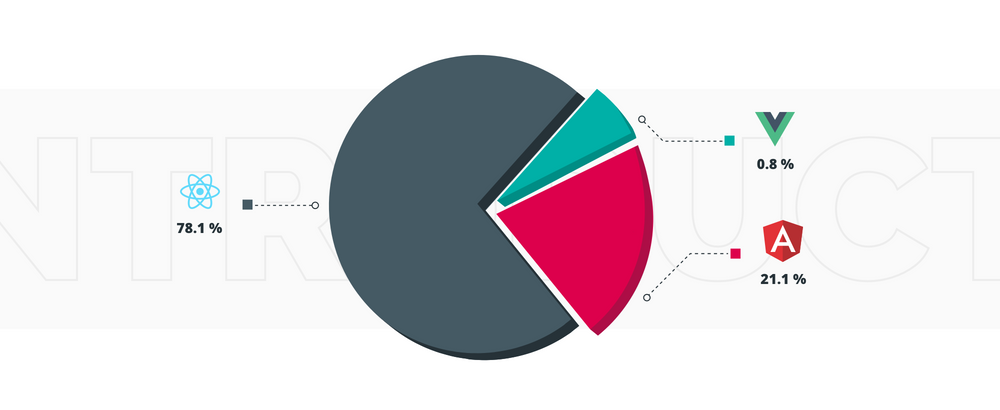
\includegraphics[width=0.80\textwidth]{pics/AngularReactVue.png}
    \caption{Marktanteil}
    \label{fig:angular_react_vue}
\end{figure}

Da der Auftrag in einer Progressive-Web-App besteht, war klar, dass eine JavaScript-Anwendung die Anforderungen der ÖBB am besten
abdecken würde. In dieser Grafik werden die Marktanteile der drei am häufigsten benutzten JavaScript-Frameworks für
Webanwendungen dargestellt. Im folgenden gehen wir weiter auf diese drei Frameworks ein \cite{framweokrs}.

\subsection{ReactJS}
ReactJS ist eine Open-Source JavaScript Bibliothek, welche von Facebook zur Verfügung gestellt wird.

\subsubsection{Vorteile}
\begin{itemize}
    \item leicht zu lernen
    \item hohe Flexibilität
    \item viele Updates durch den hohen Marktanteil
\end{itemize}

\subsubsection{Nachteile}
\begin{itemize}
    \item wenig offizielle Dokumentation
    \item \dq zu viel Auswahl\dq
\end{itemize}

\subsection{Angular}
Angular ist ein auf TypeScript [\ref{typescript}] basierendes Open-Source Framework von Google zur Erstellung von Webanwendungen. 
\cite{angular1} \cite{angular2}

\subsubsection{Vorteile}
\begin{itemize}
    \item einheitliche Struktur, woraus sich sauberer und gut lesbarer Code ableitet
    \item Vielzahl von Bibliotheken
    \item Modularisiert
    \item Aufgebaut als Single-Page-Anwendung
\end{itemize}

\subsubsection{Nachteile}
\begin{itemize}
    \item schlechte Unterstützung in alten Browsern
    \item Nicht gut skalierbar
    \item höhere Test- und Buildzeiten
\end{itemize}

\subsection{Vue.js}
Vue.js ist ein clientseitiges JavaScript-Framework zur Erstellung von anpassungsfähigen Single-Page-Anwendungen.

\subsubsection{Vorteile}
\begin{itemize}
    \item Detaillierte Dokumentation
    \item Hohe Anpassungsfähigkeit
    \item Sehr gut skalierbar
    \item Winzige Größe
\end{itemize}

\subsubsection{Nachteile}
\begin{itemize}
    \item Große Teile der Dokumentation noch in Chinesisch
    \item Wenig Wissensaustausch bedingt durch den niedrigen Marktanteil
\end{itemize}

Aufgrund gründlicher Eavluierung der oben genannten Vor- und Nachteile und gemeinsamer Rücksprache mit dem ÖBB Technischen
Service Linz wurde sich für diese Arbeit für Angular entschieden.

\section{Angular}
Wie oben beschrieben ist Angular ein auf TypeScript basierendes Open-Source Framework, welches von Google entwickelt wird.
Angular beinhaltet neben der reinen Entwicklungs-API auch Codegeneratoren und vordefinierte Architektur-Konzepte.

\subsection{Aufbau des Angular-Frameworks}
\begin{figure}[h]
    \centering
    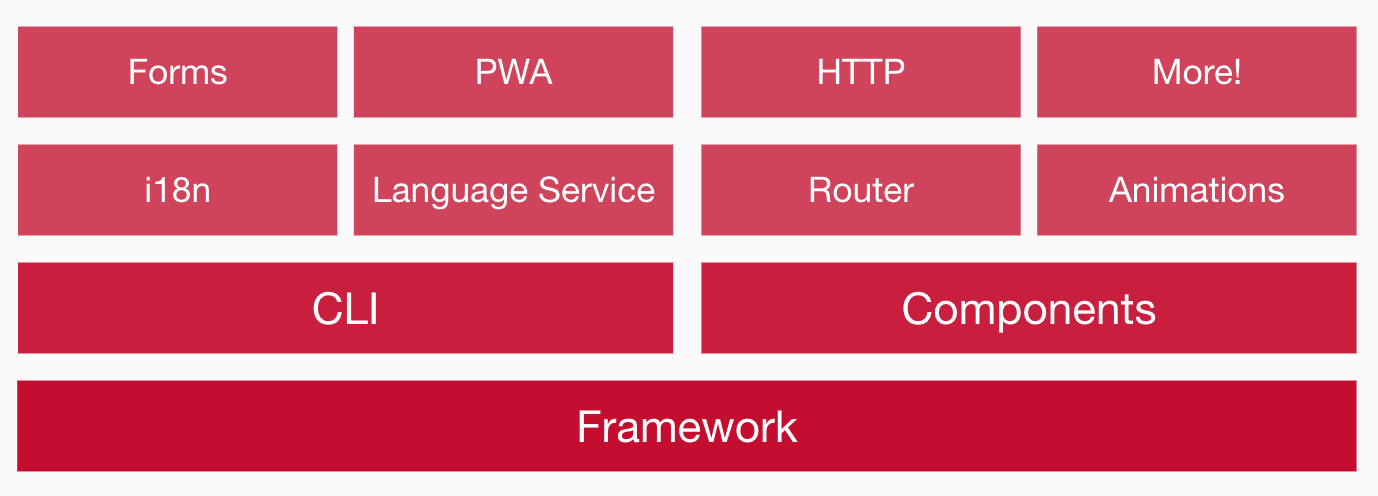
\includegraphics[width=0.80\textwidth]{pics/angular-platform-overview.png}
    \caption{Aufbau des Angular-Frameworks}
    \label{fig:aufbau_angular_framework}
\end{figure}

Die Basis von Angular bildet das Core-Framework. In diesem Framework sind die Grundkonzepte für moderne Webentwicklung 
implementiert. Darunter stehen die Angular-CLI, die Angular Komponenten und die Angular Services und darunter stehen wiederum 
kleinere, einzelne Module, die optional in die Applikation eingebunden werden können. Unter diese Module fallen beispielsweise
das Progressive Web App Modul, was in diesem Projekt benutzt wird um die Offlinefähigkeiten der Anwendungen zur Verfügung
zu stellen oder das Router Modul, welches benutzt wird um zwischen den verschiedenen Komponenten zu wechseln.

Die Angular CLI wird benutzt, um die benötigten Strukturen der Applikation zu generieren. Mit dem Befehl \lstinline |ng new "name"|
wird beispielsweise ein neues Angular-Projekt erstellt, mit \lstinline |ng generate component "name"| wird eine neue Komponente in 
dem eben generierten Projekt erstellt.

Angular Komponenten sind die Anzeigeelemente einer Anwendung. Für jede Funktion, die in der Anwendung benötigt wird, wird eine
eigene Komponente erstellt, welche wiederum aus einer TypeScript-Datei, einer HTML-Datei und einem Stylesheet bestehen. 
Sollte es notwendig sein, lassen sich diese Komponenten untereinander auch leicht verschachteln. \cite{angular4}
\begin{figure}[h]
    \centering
    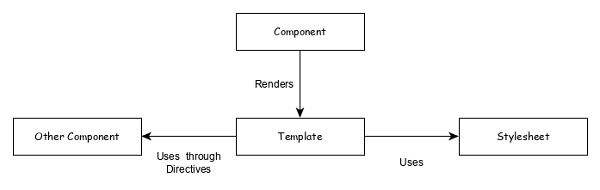
\includegraphics[width=0.80\textwidth]{pics/angular-component.jpg}
    \caption{Aufbau einer Komponente}
    \label{fig:aufbau_component}
\end{figure}

Die Komponente, beziehungsweise die TypeScript-Datei, rendert die HTML-Datei, die wiederum den Stylesheet benutzt. Andere 
Komponenten können durch importieren in der TypeScript-Datei benutzt werden.


Angular Services werden benutzt, um Logik und Daten, die nicht an einzelne Komponenten gebunden sind, herauszunehmen um 
Codeverdopplung zu vermeiden. Beispielsweise werden Daten, die in mehreren Komponenten benötigt werden, in einem Service 
gespeichert und in den Komponenten werden diese Daten dann von dem Service aus aufgerufen.
\cite{angular3}


\subsection{TypeScript} \label{typescript}
TypeScript ist, im Gegensatz zu JavaScript, statisch typisiert. Daher werden Typfehler schon in der Entwicklungszeit aufgezeigt.
TypeScript ist ein Superset von JavaScript, was aufgeteilt wird in die JavaScript Syntax, die Typisierung und das Laufzeitverhalten.

\subsubsection{Syntax}
Da, wie oben gesagt TypeScript ein Superset von JavaScript ist, ist auch jede Syntax eines JavaScript-Codes legal in 
TypeScript-Code. Code wie zum Beispiel \lstinline |let name = (Max | beinhaltet durch die fehlende Klammer einen Syntaxfehler, was aber
in JavaScript-Syntax legal ist und daher auch in TypeScript funktioniert. Dadurch kann jeder JavaScript-Code einfach in eine
TypeScript-Datei kopiert werden und es funktioniert.

\subsubsection{Typisierung}
TypeScript ist, wie oben genannt, stark typisiert, das heißt es werden verschiedene Regeln hinzugefügt, welche Werte man wann und
bei welchen Objekten nutzen kann. Würde man zum Beispiel Code wie \lstinline | x = 10 / 'hallo' | ausführen, würde es einen Fehler
werfen, da auf der rechten Seite einer mathematische Funktion kein String stehen darf. Die Stärke dieser Typisierung lässt sich mit
verschiedenen Einstellung anpassen. Sobald der Compiler den Code fertig nach Typen gecheckt hat, werden diese Typen beim 
Kompilationsvorgang gelöscht, um wieder zu einfachen JavaScript-Code zu kommen.

\subsubsection{Laufzeitverhalten}
TypeScript bewahrt das Laufzeitverhalten von JavaScript, das heißt wenn Code von JavaScript zu TypeScript geändert wird, funktioniert 
der ausgeführte Code komplett gleich.\cite{typescript1}

\subsubsection{Funktionen von TypeScript:}
\begin{itemize}
    \item TypeScript wird zu normalen JavaScript konvertiert, da TypeScript-Code nicht von Browsern interpretiert werden kann.
    Durch diese Transpilieren genannte Konvertierung kann TypeScript-Code von Browsern angezeigt werden.
    \item JavaScript kann durch das ändern der Dateiendung von .js auf .ts direkt auf TypeScript konvertiert werden.
    \item TypeScript kann in jeder Umgebung, Browser, oder Betriebssystem benutzt werden
    \item JavaScript-Bibliotheken können ohne Probleme in TypeScript-Programmen benutzt werden \cite{typescript2}
\end{itemize}

\section{Visual Studio Code}
Visual Studio Code ist die IDE, welche für die Frontendentwicklung dieser Anwendung eingesetzt wird. Es ist ein mächtiger
Code Editor welcher auf dem Desktop von Windows, Linux oder macOS läuft. In diesem Editor integriert ist Support für 
beispielsweise TypeScript und JavaScript, was aber über Extensions auf so gut wie jede häufig benutzte Programmiersprache
(CSharp, C++, Java, ...) erweitert werden kann. 

Die eingebaute IntelliSense stellt einem Funktionen für Autokomplettierung und Syntaxhervorhebung zur Verfügung, debuggen 
kann direkt in dem Editor durchgeführt werden. Git-Befehle sind ebenfalls in Visual Studio Code integriert, was die
Versionskontrolle und Zusammenarbeit mit dem Projektteam erleichtert.

Außerdem kann Visual Studio Code durch verschiedene Extensions komplett angepasst werden. Die wichtigsten darunter sind
zum Beispiel die oben genannten Extensions für andere Programmiersprachen, Extensions für Docker und Extensions für andere
Themes. \cite{vs}
